\documentclass[technicalreport]{ieicej}
%\documentclass[technicalreport,usejistfm]{ieicej}
\usepackage[dvipdfmx]{graphicx}
\usepackage{latexsym}
%\usepackage[fleqn]{amsmath}
\usepackage{amsmath}
\usepackage{amssymb}
\usepackage{multirow,eepic}
\usepackage{cite}
\usepackage{mediabb}
\usepackage{url}
\usepackage{comment}
\usepackage{epsfig}
\usepackage{subfig}
\setlength{\oddsidemargin}{-9mm}
\setlength{\evensidemargin}{-9mm}
\setlength{\topmargin}{-4mm}
%\renewcommand{\topfraction}{1.0}
%\renewcommand{\bottomfraction}{1.0}
%\renewcommand{\dbltopfraction}{1.0}
%\renewcommand{\textfraction}{0.01}
%\renewcommand{\floatpagefraction}{1.0}
%\renewcommand{\dblfloatpagefraction}{1.0}
\setcounter{topnumber}{5}
\setcounter{bottomnumber}{5}
\setcounter{totalnumber}{10}

\newcommand{\sij}{(i,j)}
\newcommand{\sijk}{(i,j,k)}
\newcommand{\mN}{{\mathcal N}}
\newcommand{\pijk}{p^{(i,j,k)}}
\newcommand{\rd}{r^{\sij}_{\rm d}}
\newcommand{\ru}{r^{\sij}_{\rm u}}
\newcommand{\rijk}{r^{(i,j,k)}}
\newcommand{\etau}{\eta_{\rm u}^{(j)}}
\newcommand{\mthc}{\mathcal C}
\def\coloneqq{\mathrel{\mathop:}=}

\jtitle{上りOFDMA適用による全二重通信無線LANの遅延時間削減}
%\jsubtitle{}
\etitle{Delay Reduction of In-Band Full-Duplex wirless LAN using Uplink OFDMA system}
%\esubtitle{}
 \alignorder=4
 \breakauthorline{4}

\authorlist{%
 \authorentry[info16@imc.cce.i.kyoto-u.ac.jp]{飯田 直人}{Naoto Iida}{^1}
 \authorentry{西尾 理志}{Takayuki NISHIO}{^1}
 \authorentry{守倉 正博}{Masahiro MORIKURA}{^1}
 \authorentry{山本 高至}{Koji YAMAMOTO}{^1}
 \authorentry{鍋谷 寿久}{Toshihisa Nabetani}{^2}
 \authorentry{青木 亜秀}{Tsuguhide Aoki}{^2}
 }

\affiliate[^1]{京都大学大学院情報学研究科\hskip1zw
  〒606-8501 京都市左京区吉田本町}
 {Graduate School of Informatics, Kyoto University\hskip1em
  Yoshida-honmachi, Sakyo-ku, Kyoto,
  606-8501 Japan}
\affiliate[^2]{株式会社東芝 研究開発センター\hskip 1zw 〒212-8582 神奈川県川崎市幸区小向東芝町1}
  {Corporate Research \& Development Center, TOSHIBA Corporation\hskip1em
   1 Komukaitoshiba-cho, Saiwai-ku, Kawasaki-shi, Kanagawa 212-8582, Japan}

\begin{document}
\begin{jabstract}
	無線LANの大容量化に向けて,自己干渉除去技術により送信と受信を同一帯域で同時に行う全二重通信無線LANが有望である.
	特に,1台のAP(Access Point)とAPへの上り通信を行うSTA(Station),
	APからの下り通信を受信するSTAの3台によるUFD(user-multiplexing Unidirectional Full-Duplex)通信は自己干渉除去技術を持たないSTAにも適用可能であるという利点がある.
	従来方式のUFD通信では,STAの送信頻度が低下し,STAが行う上り通信の遅延時間が大きくなってしまうという問題がある.
	これは,下りのTCP通信に対して返送されるTCP-ACKの遅延が増大し,TCPスループットを低下させる恐れがある.
	本稿ではこの問題の解決のために,UFD通信とOFDMAを組み合わせる方式を提案する.
	半二重通信とUFD通信を併用する従来方式にOFDMAを加え,半二重通信,UFD通信,OFDMA,UFD通信とOFDMAの組み合わせの4方式を用いる.
	遅延時間を考慮した最適化問題を設計し,それを解くことで,確率的に4つの通信方式の選択と通信に参加するSTAの選択を行う.
	本手法の有効性を計算機シミュレーションにより評価する.
\end{jabstract}
\begin{jkeyword}
	全二重通信無線LAN,ユーザ間干渉,遅延時間, OFDMA
\end{jkeyword}
\begin{eabstract}
	Self-interference cancellation techniques enable in-band full-duplex wireless local area networks (WLANs), where transmit and receive simultaneously in the same frequency band.
	In particular, user-multiplexing unidirectional full-duplex (UFD) communication, where a full-duplex access point (AP) transmits a frame to a station (STA) and receives a frame from another STA, is a promising technology for broadband WLANs, since UFD is applicable for the conventional STAs without self-interference cancellation capability.
	However, the UFD communication causes a long data frame transmission delay.
	This probrem decreases the transmission control protocol (TCP) throughput because TCP-acknowledgement (ACK) frames delay.
	In this paper, we propose a scheme to reduce the date frame transmission delay of STAs.
	The scheme uses the UFD communication and uplink OFDMA system, and increases transmission opportunities of STAs.
	Simulation results show that the scheme reduce the delay which is the same level with the half-duplex system.

\end{eabstract}
\begin{ekeyword}
	full-duplex wireless LAN, inter-user interference, delay, OFDMA
\end{ekeyword}

\titlepagebaselinestretch{0.95}

\maketitle

\section{はじめに}
	近年,無線LAN(Local Area Network)が急速に普及し,急増するトラヒックにより2.4\,GHz帯は逼迫しており,
	近い将来5\,GHz帯の逼迫も懸念されることから,無線LANのさらなる大容量化は急務である.
	大容量化を実現する方法の一つとして,送信と受信を同じ周波数帯で同時に行う全二重通信無線LANが有望である.
	全二重通信無線LANでは上り通信と下り通信を同一帯域で同時に行うため,システムスループットを向上させることができる.
	全二重通信無線LANには,図\ref{fig:topology}\subref{fig:bfd}のようなAP(Access Point)の送信先STA(station)とAPへの上り通信を行うSTAが同じである双方向全二重(BFD: Bidirectional Full-Duplex)通信と,
	図\ref{fig:topology}\subref{fig:ufd}に示すような上り通信を行うSTAと下り通信を受信するSTAが異なる全二重(UFD: user-multiplexing Unidirectional Full-Duplex)通信がある.
	UFD通信は半二重通信にしか対応していないSTAにも適用可能であるという利点がある.
	このUFD通信を用いた無線LANでは二つの干渉が問題となる.
	一つは,送受信を行っているAPにおいて,送信信号が所望の受信信号に干渉を及ぼす自己干渉である.
	自己干渉を受けるAPにとって干渉波は自身の送信信号であり既知であるため,
	自己干渉除去技術を用いて自己干渉を最大110\,dB除去できることが示されている~\cite{fdmac, stanford1}.
	もう一つは,STA $j$の送信信号がもう一方のSTA $i$の受信信号に干渉を及ぼすユーザ間干渉である.
	ユーザ間干渉では,干渉を受けるSTA $i$にとって干渉波がSTA $j$の送信する未知の信号であるため,
	自己干渉のように除去することができない.
	\par
	このユーザ間干渉の影響を低減するためには,干渉の大きさを考慮して上り通信を行うSTAと下り通信を受信するSTAの適切な組み合わせを選択することが必要である.
	我々はUFD通信におけるSTA選択を最適化問題として定式化し,システムスループットとSTA間の送信機会に関する公平性を両立させる手法を提案している~\cite{promac_fair}.
	\par
	しかし,UFD通信では半二重通信を用いる場合に比べ,上り通信を行うSTAの遅延時間が増大してしまうという課題が残っている.
	これは,半二重通信の場合と比べて下り通信を行うAPの通信比率が増え,上り通信を行うSTAの送信機会が減少するためである.
	上り通信の遅延時間が増大すると,TCP(Transmissioin Control Protocol)の下り通信に対して返送されるTCP-ACK(Acknowledgement)の送信が遅れ,
	その結果,下り通信のTCPスループットが低下する恐れがある.
	\par
	本稿では,遅延時間削減のために図\ref{fig:ofdma}のようにUFD通信に加え,
	上り通信にOFDMA(Orthogonal Frequency-Division Multiple Access)を用いるためのSTA選択手法を提案する.
	OFDMAとは周波数チャネルを複数に分割し,サブキャリアを複数のユーザに割り当て,並列に伝送する方式である.
	現在策定が進められているIEEE 802.11axにおいて,OFDMAは,短いフレームの並列伝送による周波数利用効率の向上や,
	TCP-ACKの遅延時間削減によるTCPスループットの向上を実現する技術として期待されている.
	提案方式では,このOFDMAによって上り通信を多重化しSTAの送信頻度を増加させ,遅延時間を削減する.
	~\cite{promac_fair}における最適化問題,STA選択手法をOFDMAを適用できるように拡張し,
	半二重通信,UFD通信,OFMDA通信,UFD通信とOFDMA通信の組み合わせの4つの方式を切り替え,STA選択を行う手法を提案する.
	本手法の有効性を計算機シミュレーションにより評価する.
	\par
	本稿の構成は以下のとおりである.第2章で本稿で扱うシステムモデルについて述べ,
	第3章では従来方式の問題点について述べる.
	更に,第4章において提案方式について述べ,第5章では提案方式の有効性をシミュレーションによって評価する.
	最後に第6章でまとめとする.

	\begin{figure}[t]
		\centering
		\subfloat[BFD通信]{
			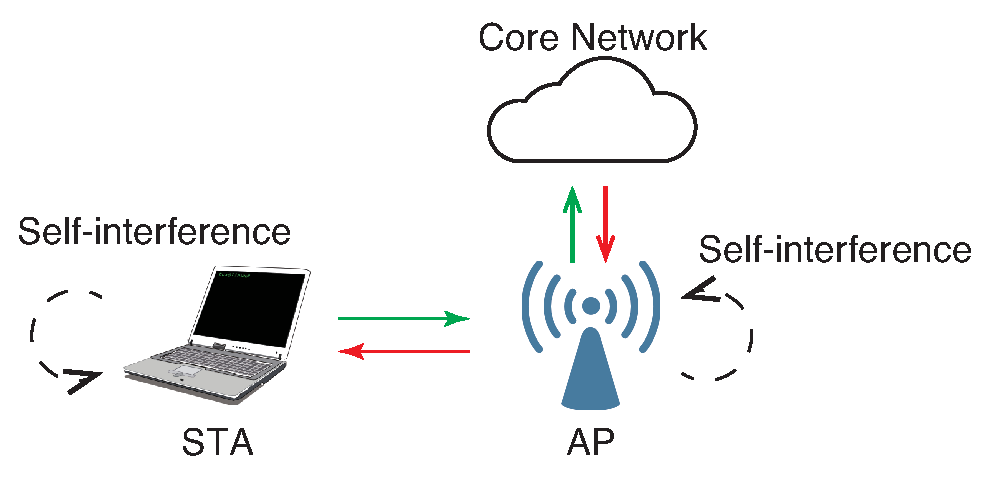
\epsfig{file=fig/bfd.eps, scale=0.4}
			\label{fig:bfd}
		}
		\\
		\subfloat[UFD通信]{
			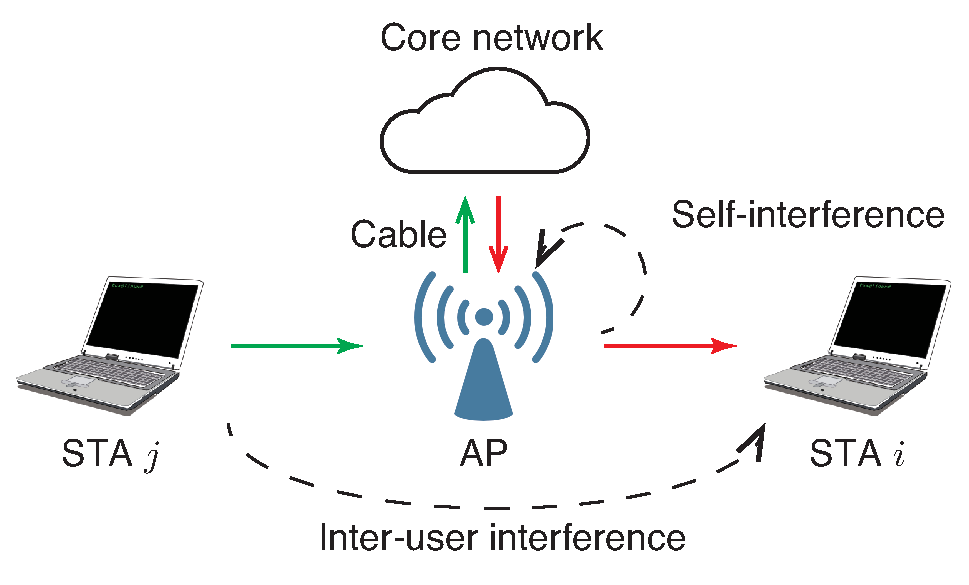
\epsfig{file=fig/ufd.eps, scale=0.4}
			\label{fig:ufd}
		}
		\caption{全二重通信の適用例}
		\label{fig:topology}
	\end{figure}

	\begin{figure}[t]
		\centering
		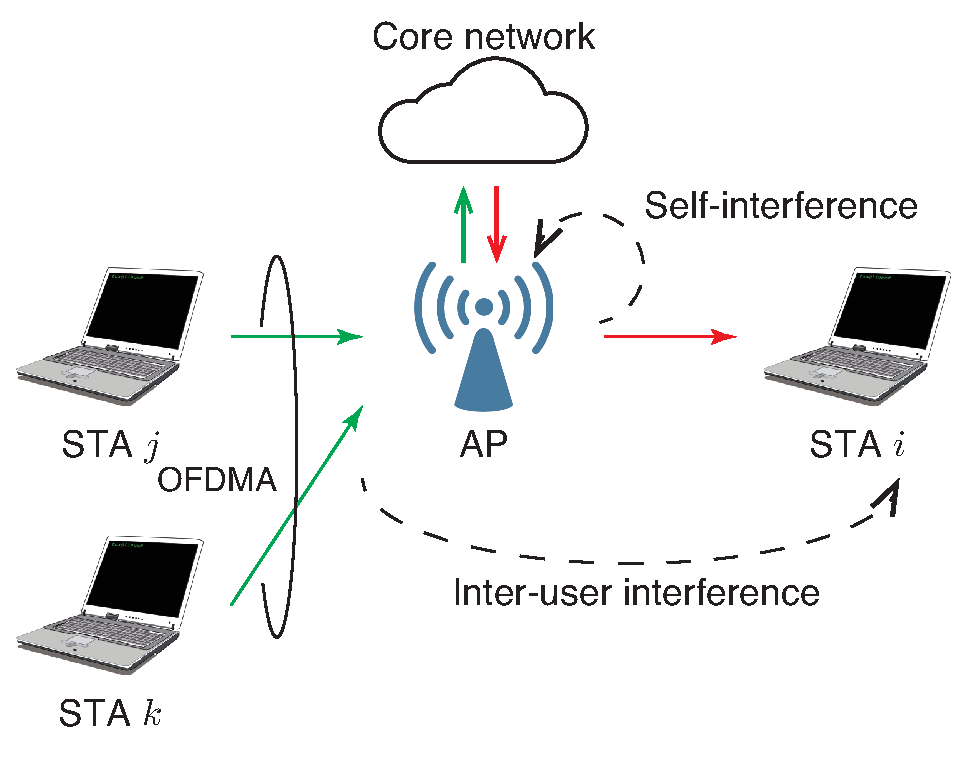
\epsfig{file=fig/ofdma.eps, scale=0.4}
		\caption{UFD通信とOFDMAの組み合わせ}
		\label{fig:ofdma}
	\end{figure}

\section{システムモデル}\label{seq:system}
	\begin{figure}[t]
		\centering
		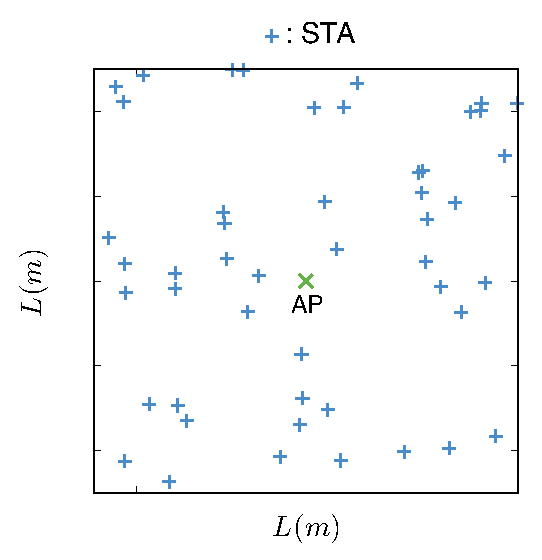
\epsfig{file=fig/pos.eps, scale=0.6}
		\caption{システムモデル(中心に設置されたAPとランダムに配置されたSTA)}
		\label{fig:model}
	\end{figure}

	本稿で検討するシステムモデルを図\ref{fig:model}に示す.
	1台のAPが$L$\,m四方の領域の中心に設置され,その周りに$N$台のSTAがランダムに配置されているとする.
	それらSTAのインデックス集合を$\mN=\{1,2,...,N\}$とする.
	OFDMAによる多重化は二多重までとし,
	この$N$台のSTAの中から,図\ref{fig:topology}\subref{fig:ofdma}のようにAPからの下り通信を受信するSTA $i$と,
	APへの上り通信を行うSTA $j$,$k$を選び出す.
	このとき,STAの組み合わせを$\sijk$と表現し,$i,\ j,\ k \in \{0\}\cup \mN$であり,
	STAは自己干渉除去技術を持たずBFD通信はできないと仮定して$i\neq j$かつ$i\neq k$とする.
	また,$i$,$j$,$k$のすべてが0になることはないものとする.
	$i$,$j$,$k$のそれぞれが取る値によって以下の通信方式を示し,切り替え可能であるものとする.
	\begin{description}
		\item[\hspace{15pt}$i=0\cap ((jk=0 \cap j+k\neq0) \cup(j=k\neq0))$の場合]\mbox{}\\
			\hspace{30pt}上りの半二重通信
		\item[\hspace{15pt}$i\neq0 \cap j=k=0$の場合]\mbox{}\\
			\hspace{30pt}下りの半二重通信
		\item[\hspace{15pt}$i\neq0 \cap ((jk\neq0 \cap j+k\neq0) \cup (j=k\neq0))$の場合]\mbox{}\\
			\hspace{30pt}UFD通信
		\item[\hspace{15pt}$i=0 \cap jk\neq0 \cap j\neq k$の場合]\mbox{}\\
			\hspace{30pt}上りOFDMA
		\item[\hspace{15pt}$i\neq0 \cap j\neq0 \cap k\neq0$の場合]\mbox{}\\
			\hspace{30pt}OFDMAとUFD通信の組み合わせ
	\end{description}
	\par
	また,STAの組み合わせを決定する際に用いる推定スループットには,上り下り通信のそれぞれのSINR(Signal-to-Interference plus Noise power Ratio)から求めた以下のシャノン容量$C$を用いる.
	\begin{equation}
		C=B\log_2(1+{\rm SINR}) \label{eq:capacity}
	\end{equation}
	ただし,$B$は通信に用いる帯域幅である.
	\par
	本稿では,遅延時間の指標として送信待機時間を用いる.
	送信待機時間とは,STAにおいてあるデータフレームがバッファの先頭に到着してから送信が開始されるまでの時間とする.
	これは,データフレームがバッファに到着してから先頭に来るまでの時間はトラヒックやバッファサイズ,輻輳制御によって変動することから,
	無線LANでの通信方式による遅延時間の違いを知るためにはこれらを除く必要があるためである.



%\section{従来方式の問題点とその原因}\label{sec:problem}
%	従来のUFD通信を用いる方式では,半二重通信である場合に比べて遅延時間が増大してしまう.
%	本節では遅延時間の増加という問題点とその原因について述べる.
%	\subsection{遅延時間の増加}
%		\begin{figure}[t]
%			\centering
%			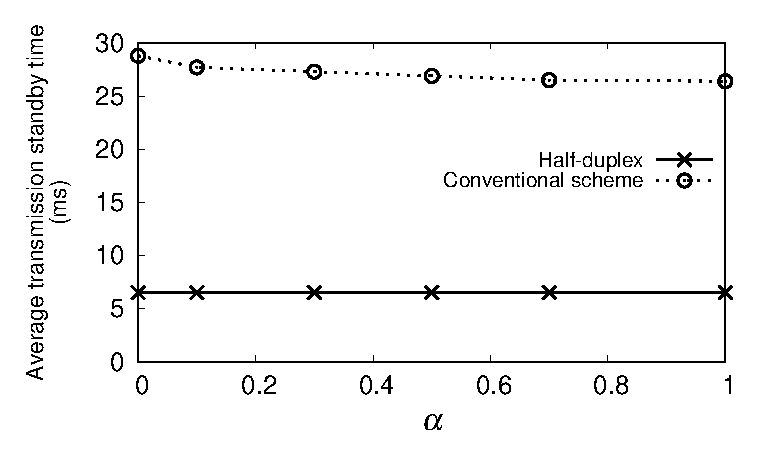
\epsfig{file=graph/delay_sub.eps, scale=0.6}
%			\caption{半二重通信と従来方式における送信待機時間}
%			\label{fig:delay_sub}
%		\end{figure}
%		図\ref{fig:delay_sub}に半二重通信のみを用いる場合と半二重通信とUFD通信を併用する従来方式~\cite{promac_fair}の場合の
%		STAの平均送信待機時間を示す.
%		ただし,送信待機時間とは各STAにおいてあるデータフレームがバッファの先頭に到着してからの経過時間であり,
%		$\alpha$は目的関数における送信待機時間の.影響を調整するパラメータである.
%		送信待機時間が半二重通信の場合と比べて,従来方式は4倍以上の値となっていることがわかる.
%	\subsection{伝送速度の低下}
%		本節では送信待機時間が半二重通信の場合と比べて大きくなってしまう原因について述べる.
%		APの送信電力を$P_{\rm AP}$,STA $j$の送信電力を$P_j$とし,
%		AP-STA $i$間,AP-STA $j$間,STA $i$-$j$間のチャネル係数をそれぞれ$h_{{\rm AP},i}$,$h_{{\rm AP},j}$,$h_{i,j}$とし,
%		雑音電力を$\sigma^2$とすると,半二重通信の場合における上下通信のSNRはそれぞれ,
%		\begin{align}
%			{\rm SNR_{\rm d}^{\rm h}} &= \cfrac{P_{\rm AP}|h_{{\rm AP},i}|^2}{\sigma^2} \label{eq:hd}\\
%			{\rm SNR_{\rm u}^{\rm h}} &= \cfrac{P_j |h_{{\rm AP},j}|^2}{\sigma^2}\label{eq:hu}
%		\end{align}
%		となる.
%		一方,UFD通信の場合の上下通信のSINRはそれぞれ,
%		\begin{align}
%			{\rm SINR_{\rm d}^{\rm f}} &= \cfrac{P_{\rm AP} |h_{{\rm AP},i}|^2}{\sigma^2+P_j'|h_{i,j}|^2}\label{eq:fd}\\
%		\end{align}
%		となる.
%		ただし,$P_j'$は~\cite{promac}による送信電力制御を行った場合のSTA $j$の送信電力であり$P_j'\leq P_j$である.
%		また,$h_{\rm AP,AP}$はAPの送信信号がAP自身によって受信されるまでの伝搬路のチャネル係数に,
%		自己干渉除去技術による干渉除去の効果を加味した値である.
%		\par
%		式\eqref{eq:hd}と\eqref{eq:fd}の比較,式\eqref{eq:hu}と\eqref{eq:fu}の比較からわかるように,
%		UFD通信における上下通信のSINRは,半二重通信の場合のSNRと比べて干渉と送信電力制御による送信電力低下の分だけ悪化する.
%		これにより,UFD通信では,半二重通信の場合に比べて上下通信それぞれの伝送速度が低下してしまう.

\section{提案方式}\label{sec:propose}
	本節では,遅延時間の増大を防ぐため,上り通信をOFDMAを用いて多重化することを提案する.
	OFDMAを用いてSTAの送信機会を増加させることで遅延時間を削減する.
	STA決定手法は従来方式~\cite{promac_fair}における手法をOFDMAを適用できるように拡張する.
	また,計算時間削減のための手法についても検討する.
	\subsection{STAの組み合わせ決定手法}\label{sec:opt}
		%まず,STAの組み合わせの集合${\mathcal C}_{\rm half}$,${\mathcal C}_{\rm UFD}$,${\mathcal C}_{\rm OFDMA}$,${\mathcal C}_{\rm OFDMA-UFD}$,${\mathcal C}$を以下のように定義する.
		%\begin{align}
		%	&{\mathcal C}_{\rm half} \coloneqq \{\sijk : i=0\cap ((jk=0 \cap j+k\neq0) \cup(j=k\neq0)),\ \rijk >\epsilon\} \\
		%	&{\mathcal C}_{\rm UFD} \coloneqq \{\sijk : i,j\in{\mathcal N},\ i\neq j,\ r^{\sij}_{\rm d},\ r^{\sij}_{\rm u}>\epsilon\} \\
		%	&{\mathcal C}_{\rm OFDMA} \coloneqq \{\sijk : i=0,\ jk\neq0\in{\mathcal N},\ r^{\sij}_{\rm d},\ r^{\sij}_{\rm u}>\epsilon\}
		%\end{align}
		APはすべての組み合わせ$(i,j,k)$に対してスループット$r^{(i,j,k)}_{\rm d}$,$r^{(i,j,k)}_{\rm u1}$,$r^{(i,j,k)}_{\rm u2}$を推定する.
		ただし,$r^{(i,j,k)}_{\rm d}$はAPからSTA $i$への下り通信の推定スループット,$r^{(i,j,k)}_{\rm u1}$,$r^{(i,j,k)}_{\rm u2}$はSTA $j$,$k$による上り通信の推定スループットである.
		ここで,全組み合わせの集合から最低伝送速度の所要SINRを満たさない通信が含まれている組み合わせを除外した集合を$\mthc$とする,
		APは$\rijk=r^{(i,j,k)}_{\rm d}+r^{(i,j,k)}_{\rm u1}+r^{(i,j,k)}_{\rm u2}$とすべてのSTAの送信待機時間$d^{(j)}$を用いて,以下の最適化問題を解き各組み合わせで通信が行われる確率$p^{(i,j,k)}$を求める.
		ただし,送信待機時間とはあるデータフレームがバッファの先頭に到着してからの経過時間である.
		\begin{align}
			&{\mathcal P}_1: && {\rm max} \sum_{(i,j,k)\in{\mathcal C}} p^{(i,j,k)}r^{(i,j,k)}(d^{(j)}+d^{(k)})^{\alpha} &&&&&&\\
			&{\rm subject\ to} && \sum_{j,k\in\{j,k:(i,j,k)\in{\mathcal C}\}} p^{(i,j,k)} \geq \eta_{\rm d}^{(i)}, \forall i\in {\mathcal N} \label{eq:etad} \\
			&&& \sum_{i,j\in\{i,j:(i,j,k)\in{\mathcal C}\}} p^{(i,j,a)} +\sum_{i,k\in\{i,k:(i,j,k)\in{\mathcal C}\}} p^{(i,a,k)} \nonumber\\
			&&&\qquad- \sum_{i\in\{i:(i,j,k)\in{\mathcal C}\}} p^{(i,a,a)} \geq \eta_{\rm u}^{(a)}, \forall a\in {\mathcal N} \label{eq:etau} \\
			&&& \sum_{(i,j,k)\in{\mathcal C}} p^{(i,j,k)}=1 \\
			&{\rm variables:} &&p^{(i,j,k)} \in {\mathbb R}_{\geq 0},\forall(i,j,k)\in {\mathcal C}
		\end{align}
		\par
		目的関数は確率$\pijk$,推定スループット$\rijk$,STA $j$,$k$の送信待機時間の和$d^{(j)}+d^{(k)}$の積となっており,
		推定スループットが大きく,送信待機時間が大きなSTAを含む組ほど通信を行う確率が高くなるよう設計されている.
		また,$\alpha$は目的関数に対する送信待機時間の影響の大小を調節するための値であり,
		大きいほど送信待機時間の大きなSTAを含む組が選ばれやすくなる.
		一つ目の制約条件はあるSTA $i$が下り通信の送信先となる確率を$\eta_{\rm d}^{(i)}$以上とする条件であり,
		二つ目はあるSTA $a$が上り通信を行う確率を$\eta_{\rm u}^{(a)}$以上とする条件である.
		$\eta_{\rm d}$,$\eta_{\rm u}$は0より大きく,それぞれのトラヒックに比例した値が設定される.
		これらは,選ばれる確率が0となるSTAが発生しないようにするための条件である.
		APによって算出された確率$\pijk$はビーコンフレームによってSTAに通知される.
		\par
		次に,STA $i$,$j$,$k$を決定する方法を述べる.
		APは以下の式に従って,各STAが下り通信の送信先となる確率$p_{\rm d}^{(i)}$を求める.
		\begin{equation}
			p_{\rm d}^{(i)}= \sum_{j,k\in\{j,k:(i,j,k)\in{\mathcal C}\}}p^{(i,j,k)},\ \forall i \in \{0\}\cup{\mathcal N}
		\end{equation}
		APはこの確率$p_{\rm d}^{(i)}$に従って確率的にSTA $i$を選択する.
		ここで下り通信の送信先として決定したSTAをSTA $i^*$とする.
		このとき$i^*=0$であれば,下り通信が行われないことを示す.
		STA $i^*$の決定後APはSTA $i^*$へ送信するデータフレームのヘッダ部分のみを送信し,送信先がSTA $i^*$であることを全STAに通知する.
		STA $i^*$以外のSTAは以下の条件付き確率を計算する.
		\begin{align}
			p_{\rm u1}^{(i^*,j,k)}=\left(\sum_{k\in\{k:(i^*,j,k)\in\mthc\}} p^{(i^*,j,k)}\right) / p_{\rm d}^{(i)}, \\
			\qquad\qquad\forall j \in \{0\}\cup{\mathcal N}\backslash \{i^*\}
		\end{align}
		これは,APがSTA $i^*$へ送信することが決まった上で,各STA $j$が上り通信を行う確率である.
		この条件付き確率をもとに,各STAはコンテンションウィンドウサイズ${\rm CW}^{\sijk}_{\rm u1}$を
		\begin{equation}
			{\rm CW}^{(i^*,j,k)}_{\rm u1} = \lceil 1/p_{\rm u1}^{(i^*,j,k)} \rceil
		\end{equation}
		と設定する.
		ただし,$\lceil x \rceil$は$x$を超えない最大の整数である.
		各STAは$[0,\ {\rm CW}^{(i^*,j,k)}_{\rm u1}]$の一様分布から生成されるバックオフカウンタ$w_{\rm u1}^{(i^*,j,k)}$を設定し,
		CSMA/CAのバックオフアルゴリズムを用いてバックオフカウンタを1ずつ減らす.
		その結果,最初にカウンタが0となったSTAが上り通信を行う.
		このSTAをSTA $j^*$とすると,STA $j^*$はAPへ送信するデータフレームのヘッダ部分のみを送信し,
		他のSTAに自身が上り通信を行うことを通知する.
		残りのSTAは,STA $j$の決定の際と同様に以下の条件付き確率を求める.
		\begin{align}
			p_{\rm u2}^{(i^*,j^*,k)}=p^{(i^*,j^*,k)} / \left(\sum_{k\in\{k:(i^*,j^*,k)\in\mthc\}} p^{(i^*,j^*,k)}\right)\\
			\qquad\qquad\forall k \in \{0\}\cup{\mathcal N}\backslash \{i^*,j^*\}
		\end{align}
		これは,STA $i^*$,STA $j^*$が通信に参加することが決まった上での各STAがSTA $k$として上り通信を行う確率である.
		以降STA $j$を決定する際と同様に${\rm CW}^{(i^*,j^*,k)}_{\rm u2}$,$w_{\rm u2}^{(i^*,j^*,k)}$を設定し,
		最小の$w_{\rm u2}^{(i^*,j^*,k)}$を設定したSTAがSTA $k^*$となり,組み合わせが決まる.
		組み合わせ決定後,AP,STA $j^*$,$k^*$はそれぞれデータフレームを送信する.

	\subsection{計算時間の削減}\label{sec:time}
		\begin{figure}[t]
			\centering
			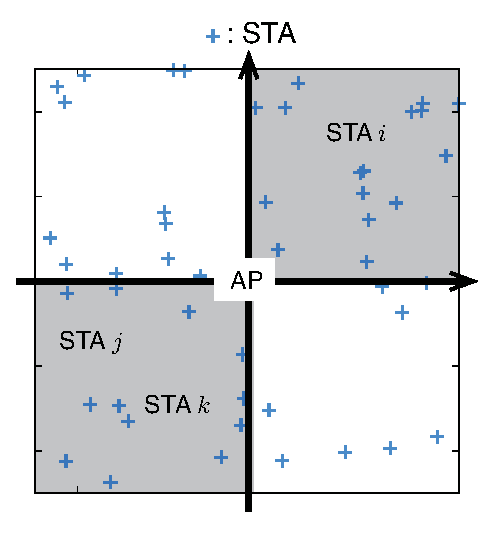
\epsfig{file=fig/time.eps, scale=0.6}
			\caption{位置によるSTAのグループ分け}
			\label{fig:time_image}
		\end{figure}
		本節では,最適化問題を解くための計算時間を削減する手法について検討する.
		APは前節の最適化問題を定期的に解いて,確率$\pijk$を更新しなければならない.
		なぜなら,目的関数に含まれる送信待機時間$d^{(j)}$,$d^{(k)}$はSTAが送信を行う度に変化する値であるためである.
		計算結果はビーコンフレームによって全STAに通知されるが,一般的なビーコン周期は100\,msであり,
		ビーコン毎に最適化問題を解く場合は最大で100\,ms以内に解かねばならず,
		仮にビーコン数回毎に更新するように計算頻度を減らしたとしても数百ミリ秒単位で解けなければならない.
		そのため,計算時間を削減することを考えなければならない.
		\par
		一般的に最適化問題の計算時間は変数の数に依存する.
		提案方式における変数は$\pijk$であり,この数は組み合わせの数$|\mthc|$と同じである.
		したがって,集合$\mthc$に含まれる組み合わせの数を減らすことができれば計算時間を削減することができる.
		最適化の結果に与える影響をできるだけ小さくしながら組み合わせの数を減らすためには,
		ユーザ間干渉が大きく,例え通信ができたとしても伝送速度が低くなってしまうような組み合わせを除けばよい.
		\par
		そこで,本稿では計算時間の削減を行うためにSTAを位置によってグループ分けを行い,その中から組み合わせを決定するという方法をとる.
		具体的には,図\ref{fig:time_image}のようにAPを中心とした直行座標を設定し,それぞれのSTAがどの象限に位置するかによって4つのグループに分ける.
		そして,組み合わせの集合$\mthc$には,OFDMAとUFD通信を組み合わせる場合はSTA $i$と2台のSTA $j$,$k$は対角の象限,STA $j$と$k$は同じ象限に存在するような組み合わせ,UFD通信の場合はSTA$i$と$j$は対角の象限に存在する組み合わせのみ含める.
		ユーザ間干渉はSTA $i$とSTA $j$,$k$の間の距離が小さいほど大きくなるため,
		STA $i$とSTA$j$,$k$が隣り合った象限に存在する組み合わせはユーザ間干渉が大きくなる可能性が高い.
		そのため,そういった組み合わせは選択される可能性が低く,選択対象から除外しても影響は小さいと考えられる.
		\par
		ただし,本稿においてはSTAの位置は既知であるとし,時間変化もないものとする.


\section{シミュレーション評価}

	\begin{table}[t]
		\centering
		\caption{シミュレーション諸元}
		\label{tab:param}
		\begin{tabular}{cc} \hline
			領域の大きさ $L$ & 100\,m \\
			伝送速度 & シャノン容量 \\
			送信電力 & 15\,dBm \\
			雑音指数 & 10\,dB \\
			周波数帯 $f$& 2.4\,GHz \\
			帯域幅 $B$ & 20\,MHz \\
			伝搬損失 & $30\log D + 40$\\
			&($D$: 送受信点間距離)\\
			自己干渉除去 & 110\,dB \\
			シミュレーション時間 & 10\,s \\\hline
		\end{tabular}
	\end{table}

	本章では提案手法の有効性をシミュレーションによって評価する.
	半二重通信のみを用いる場合,半二重通信とUFD通信を併用する従来方式~\cite{promac_fair}と,
	半二重通信,UFD通信,OFDMA,UFD通信とOFDMA通信の組み合わせの4方式を用いる提案方式を比較する.
	OFDMAによる多重化は二多重までとし,チャネル幅は二等分するものとする.
	図\ref{fig:model}のように,1台のAPが $L=$100\,m四方の領域の中心に設置され,その周りに$N$台のSTAがランダムに配置されているとする.
	第\ref{sec:opt}節で述べた部分以外のMACプロトコルは~\cite{promac}に従うものとする.
	式\eqref{eq:etad}における$\eta_{\rm d}^{(i)}$には各STA共通の$1/[(N+1)N]$を,
	式\eqref{eq:etau}における$\eta_{\rm u}^{(a)}$には各STA共通の$1/(N+1)$を設定している.
	伝送速度はIEEE 802.11aに従う.
	上下通信ともに飽和トラヒックであり,APには1500\,Bの,STAには64\,Bのデータフレームが発生しているものとする.
	これは,トラヒックのほとんどga64\,B以下の短いフレームと1500\,B付近の長さのフレームによって占めるからである~\cite{traffic}.
	また,本稿では遅延時間を送信待機時間と定義する.

	\subsection{遅延時間の削減}
		\begin{figure}[t]
			\centering
			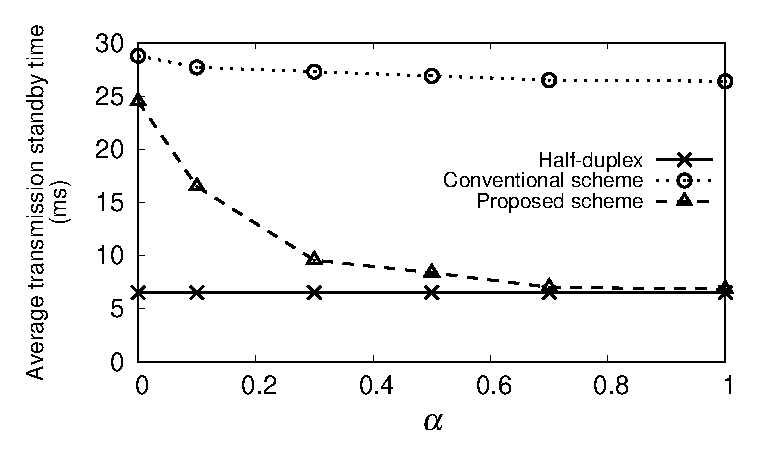
\epsfig{file=graph/delay.eps, scale=0.6}
			\caption{上り通信の遅延時間}
			\label{fig:delay}
		\end{figure}
		\begin{figure}[t]
			\centering
			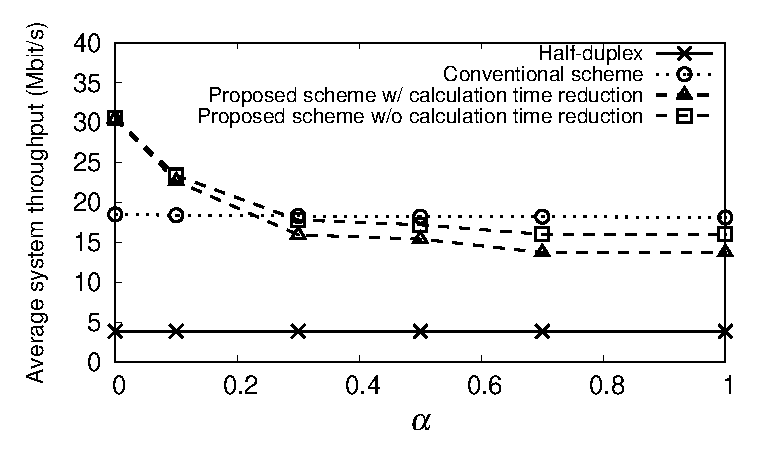
\epsfig{file=graph/thr.eps, scale=0.6}
			\caption{システムスループット}
			\label{fig:thr}
		\end{figure}

		$N=50$台の場合について,図\ref{fig:delay},\ref{fig:thr}にSTAの平均送信待機時間とシステムスループットを示す.
		半二重通信とUFD通信を用いる従来方式の送信待機時間は半二重通信のと比べ大きいことがわかる.
		一方,提案方式はパラメータ$\alpha$を大きくすることで送信待機時間を半二重通信と同等の値まで削減できていることがわかる.
		しかし,$\alpha$が大きくなるにつれて,システムスループットが低下してしまっている.
		これは,送信待機時間$d^{(j)},\ d^{(k)}$の項の影響が大きくなり,遅延時間削減を優先しているためである.
		$\alpha$を増加させ遅延時間削減を優先した結果,システムスループットは低下したものの,半二重通信に対しては3倍程度の値を維持しつつ,
		遅延時間を半二重通信と同等まで削減することができた.

	\subsection{計算時間の削減}
		\begin{table}[t]
			\centering
			\caption{最適化問題を1回解くために必要な平均時間}
			\label{tab:time}
			\begin{tabular}{cc}
			 計算時間削減なし & 計算時間削減あり\\ \hline
			 803\,ms & 483\,ms \\\hline
			\end{tabular}
		\end{table}
%		\begin{figure}[t]
%			\centering
%			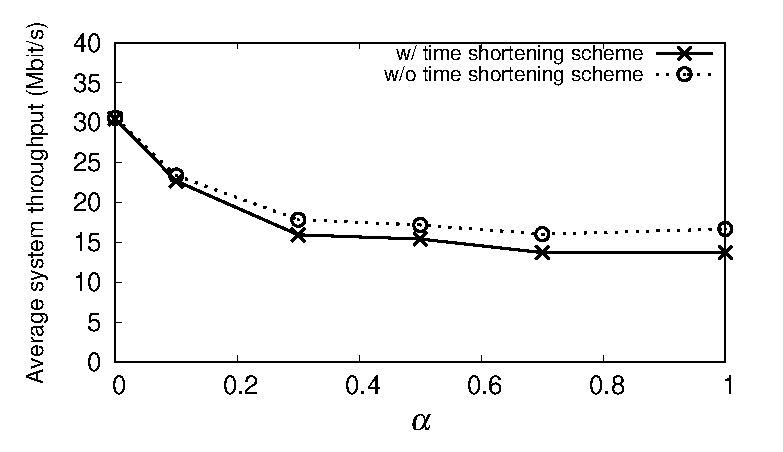
\epsfig{file=graph/thr_time.eps, scale=0.6}
%			\caption{システムスループットへの計算時間削減手法の影響}
%			\label{fig:thr_time}
%		\end{figure}

	次に計算時間について評価する.
	表\ref{tab:time}に第\ref{sec:time}節で述べた計算時間削減手法を用いた場合と用いない場合について,
	最適化問題を一回解くために必要な平均時間を示す.
	計算時間を40\%削減できている.
	さらに,計算時間削減手法を用いたことによる影響を調べるために図\ref{fig:thr}の両者のシステムスループットを比較すると,
	全体的に計算時間削減手法を用いた方が用いない場合に比べてシステムスループットが小さくなっている.
	差は$\alpha=0$のときには1\%,$\alpha=1$のときには18\%となっている.
	簡易な方式ながら大きく計算時間を削減できた.
	より高度な方式を採用することでさらなる改善が見込まれる.
%	$\alpha$が小さいときには送信待機時間$d^{(j)},\ d^{(k)}$の影響が小さく,
%	干渉の小さな組み合わせが選ばれやすい.
%	干渉の小さな組み合わせは,APに対してSTA $i$とSTA $j$,$k$が対角の位置に存在している場合であり,
%	このような組み合わせは計算時間削減手法を用いていても除外されていないため,影響が少ないと考えられる.
%	一方,$\alpha$が大きいときには送信待機時間$d^{(j)},\ d^{(k)}$の影響が大きく,
%	例えある程度干渉が大きい組み合わせでも送信待機時間が大きいSTAを選ばざる負えない.
%	このような場合は,計算時間削減手法によって除外された組み合わせの中によりよい組み合わせが含まれてしまっていることがあるため,
%	システムスループットが低下してしまうと考えられる.

\section{まとめ}
	本稿では,OFDMAとUFD通信を組み合わせて用いる手法を提案した.
	STAの遅延時間が増大するというUFD通信の問題点を,上り通信をOFDMAにより多重化し,
	STAの送信機会を増加させることで遅延時間の削減を行った.
	更に,STAのグループ分けを行い最適化問題の変数の数を減らすことで,計算時間を削減する手法についても述べた.

\bibliographystyle{sieicej}
\bibliography{main2}

\end{document}
